\chapter{Classical Visual Odometry}
\label{ch:vo}
\epigraph{Eventually, my eyes were opened, and I really understood nature.}{\textsc{Claude Monet}}

\begin{figure}[h!]
\begin{center}
		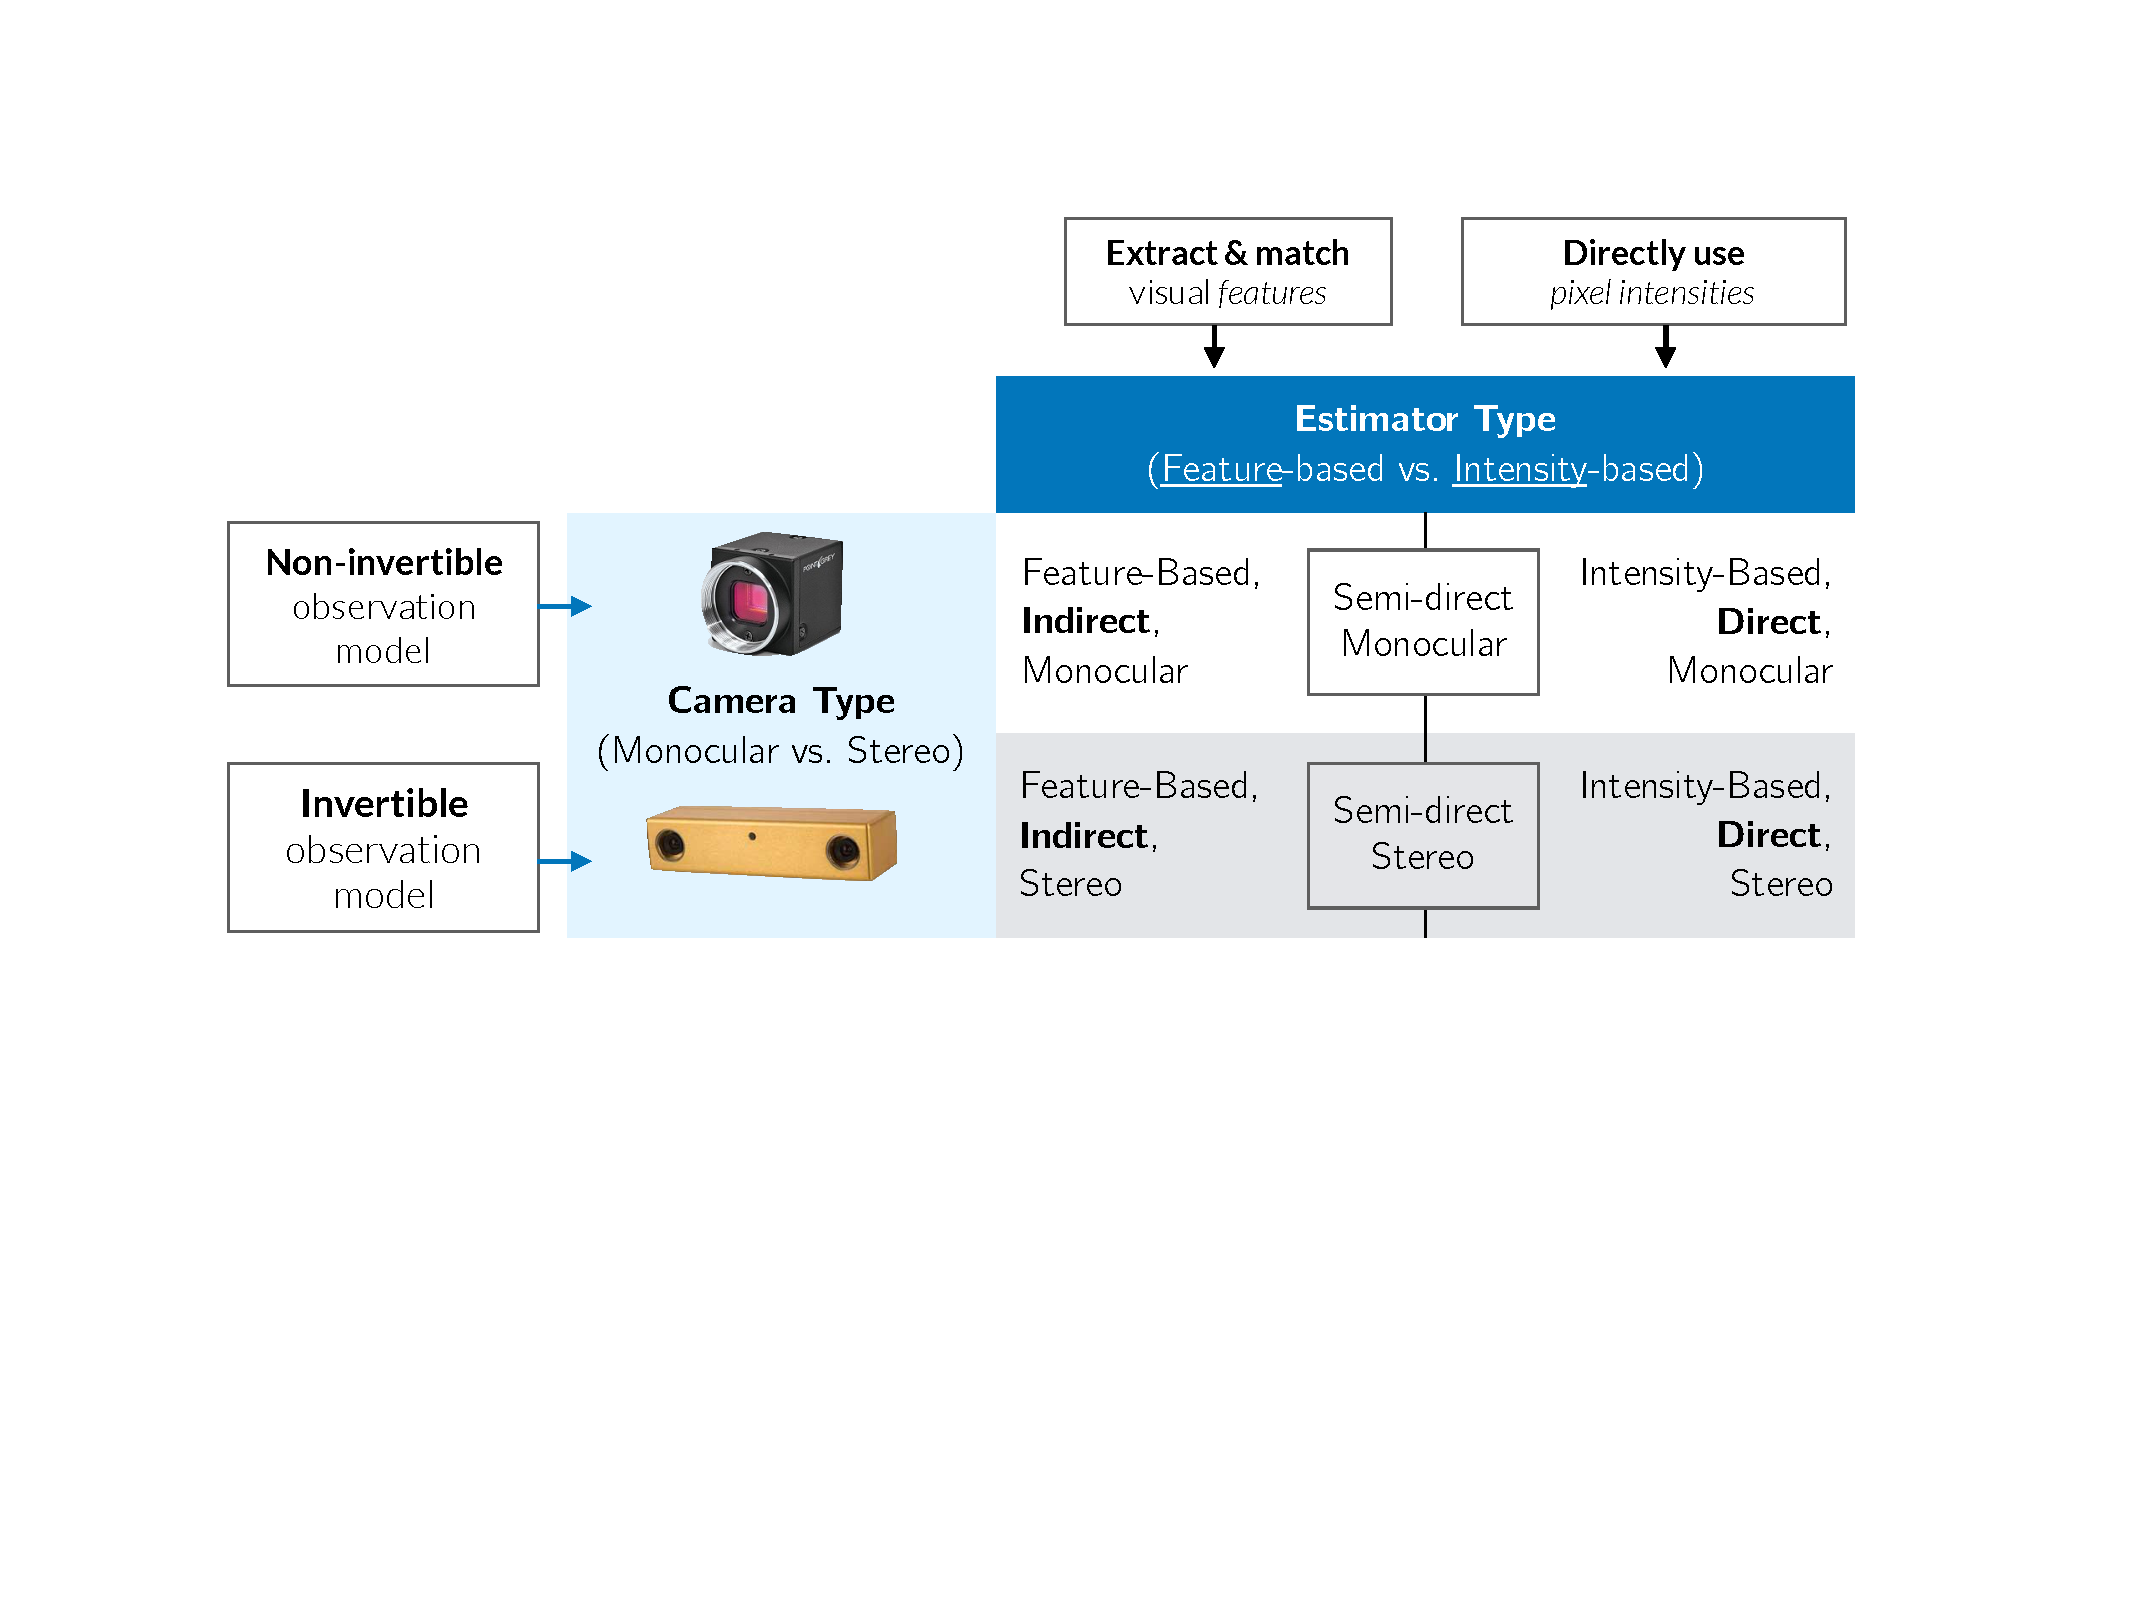
\includegraphics[width=0.95\textwidth]{classical-vo/vo_taxonomy.pdf}
		\caption{A taxonomy of different types of visual odometry.}
  	\label{fig:vo_taxonomy}
\end{center}
\end{figure}


Visual odometry (VO) has a rich history in mobile robotics and computer vision. As this dissertation largely deals with the improvement of a baseline visual odometry pipeline, we first outline the components of what we have chosen to be a canonical VO system. For a seminal tutorial on visual odometry and its more general cousin, visual SLAM, we refer the reader to \cite{Scaramuzza2011-qr,Cadena2016-ds}.
\newpage
\begin{remark}{VO Taxonomy}
VO can be largely divided along two dimensions (\Cref{fig:vo_taxonomy}): (1) the type of camera used to capture images and (2) the type of data association used to compute motion estimates. 

\textbf{Monocular vs. Stereo Camera}:
 Monocular VO methods \citep{engel_direct_2018,Tsotsos2015} use a single camera to infer motion and can use a single compact, low-power vision sensor. They do not require any extrinsic calibration but must rely on known visual cues or external information (e.g., wheel odometry, inertial measurements) to provide metric egomotion estimates. Conversely, stereo VO methods \citep{engel_direct_2018, Leutenegger2015-fk, Cvisic2015-mt} use a stereo camera to triangulate objects with metric scale. This allows stereo VO to provide metrically-accurate egomotion estimates. However, stereo methods rely on accurate extrinsic calibration, and their ability to resolve depth is limited by the baseline distance between the stereo pair and by the quality of stereo matches (which can be degraded by self-similar textures, occlusions, and foreshortening effects). 

\textbf{Direct vs. Indirect Data Association}:
The second distinction is based on the type of data association used to match sequential images and infer motion. Direct methods \citep{engel_direct_2018,wang_stereo_2017} make the assumption of brightness constancy, and attempt to find the egomotion estimate that \textit{directly} maximizes the similarity of pixel intensities between images. Indirect methods \citep{Leutenegger2015-fk,Cvisic2015-mt}, conversely, rely on image features detectors to extract a set of salient landmarks or features, and then match these landmarks across images (typically by relying on a view-invariant descriptor).	
\end{remark}



\section{Canonical VO Pipeline}

\begin{figure}[h!]
\begin{center}
		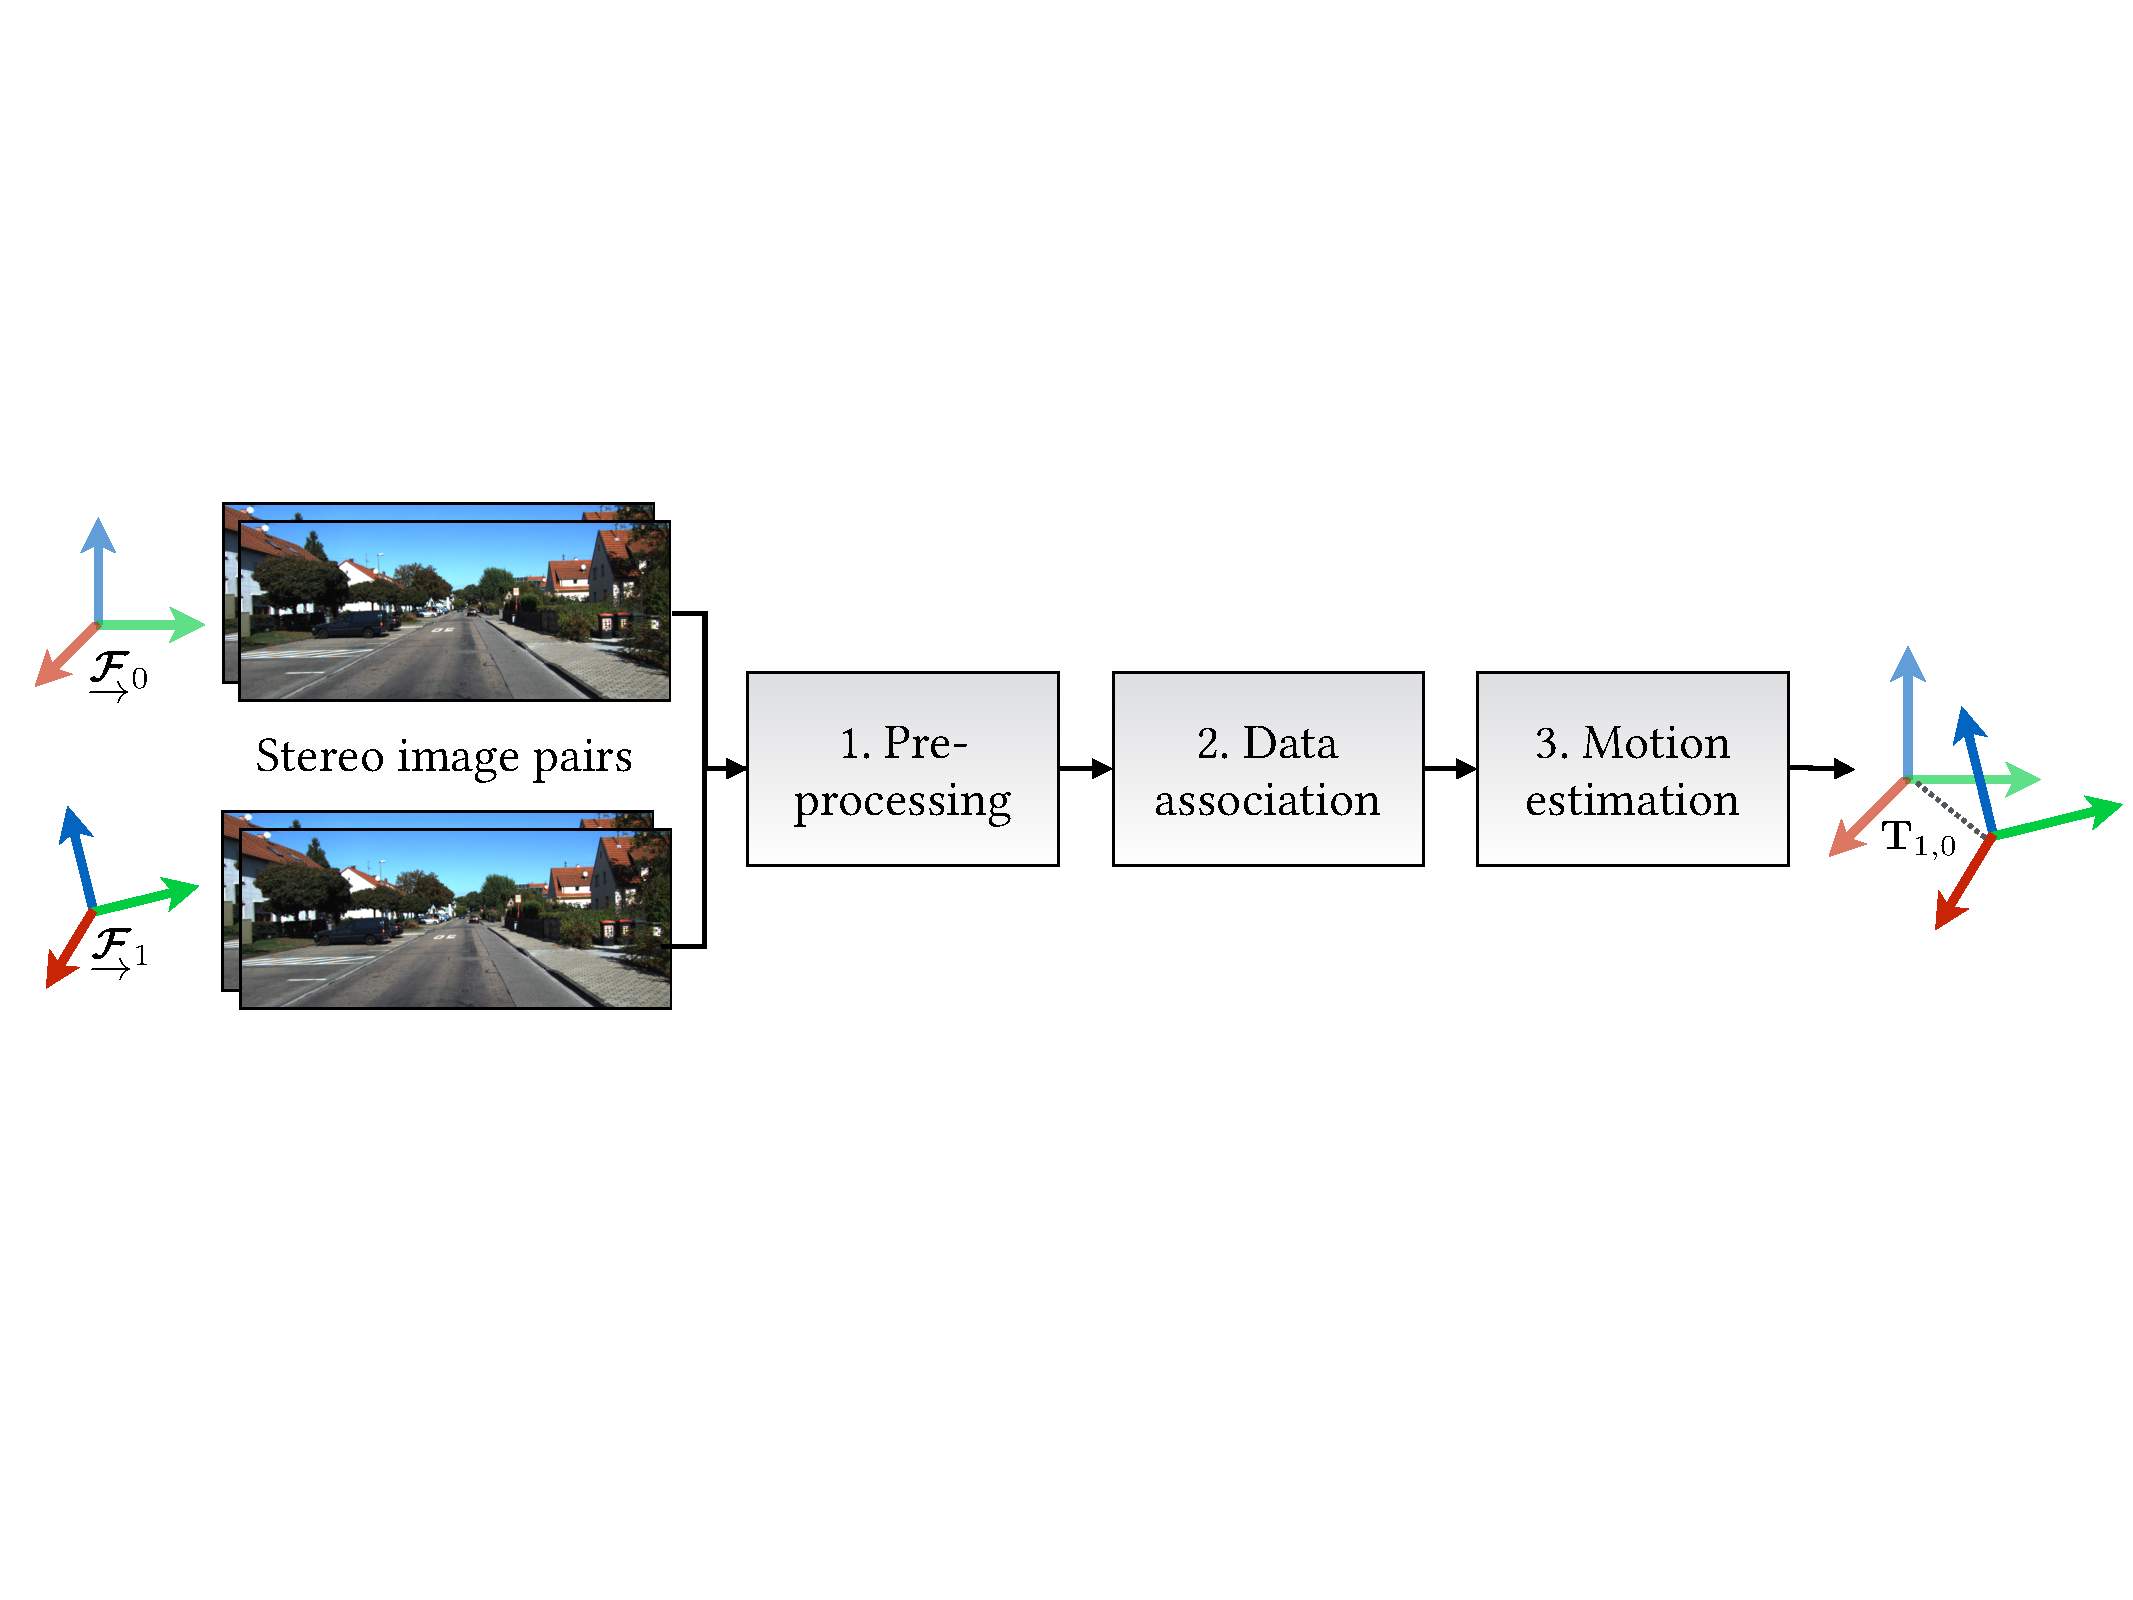
\includegraphics[width=0.98\textwidth]{classical-vo/stereo_vo_pipeline.pdf}
		\caption{A `classical' stereo visual odometry pipeline consists of several distinct components that have interpretable inputs and outputs.}
  	\label{fig:vo_stereo_vo_pipeline}
\end{center}
\end{figure}

In this dissertation, we apply our learned pseudo-sensors to a baseline stereo, indirect visual odometry pipeline (\Cref{fig:vo_stereo_vo_pipeline}). We choose this baseline system for its computational efficiency and robustness. We briefly summarize the main components of the pipeline here.



\subsection{Preprocessing}


\begin{figure}[h!]
     \centering
     \begin{subfigure}[b]{0.48\textwidth}
         \centering
         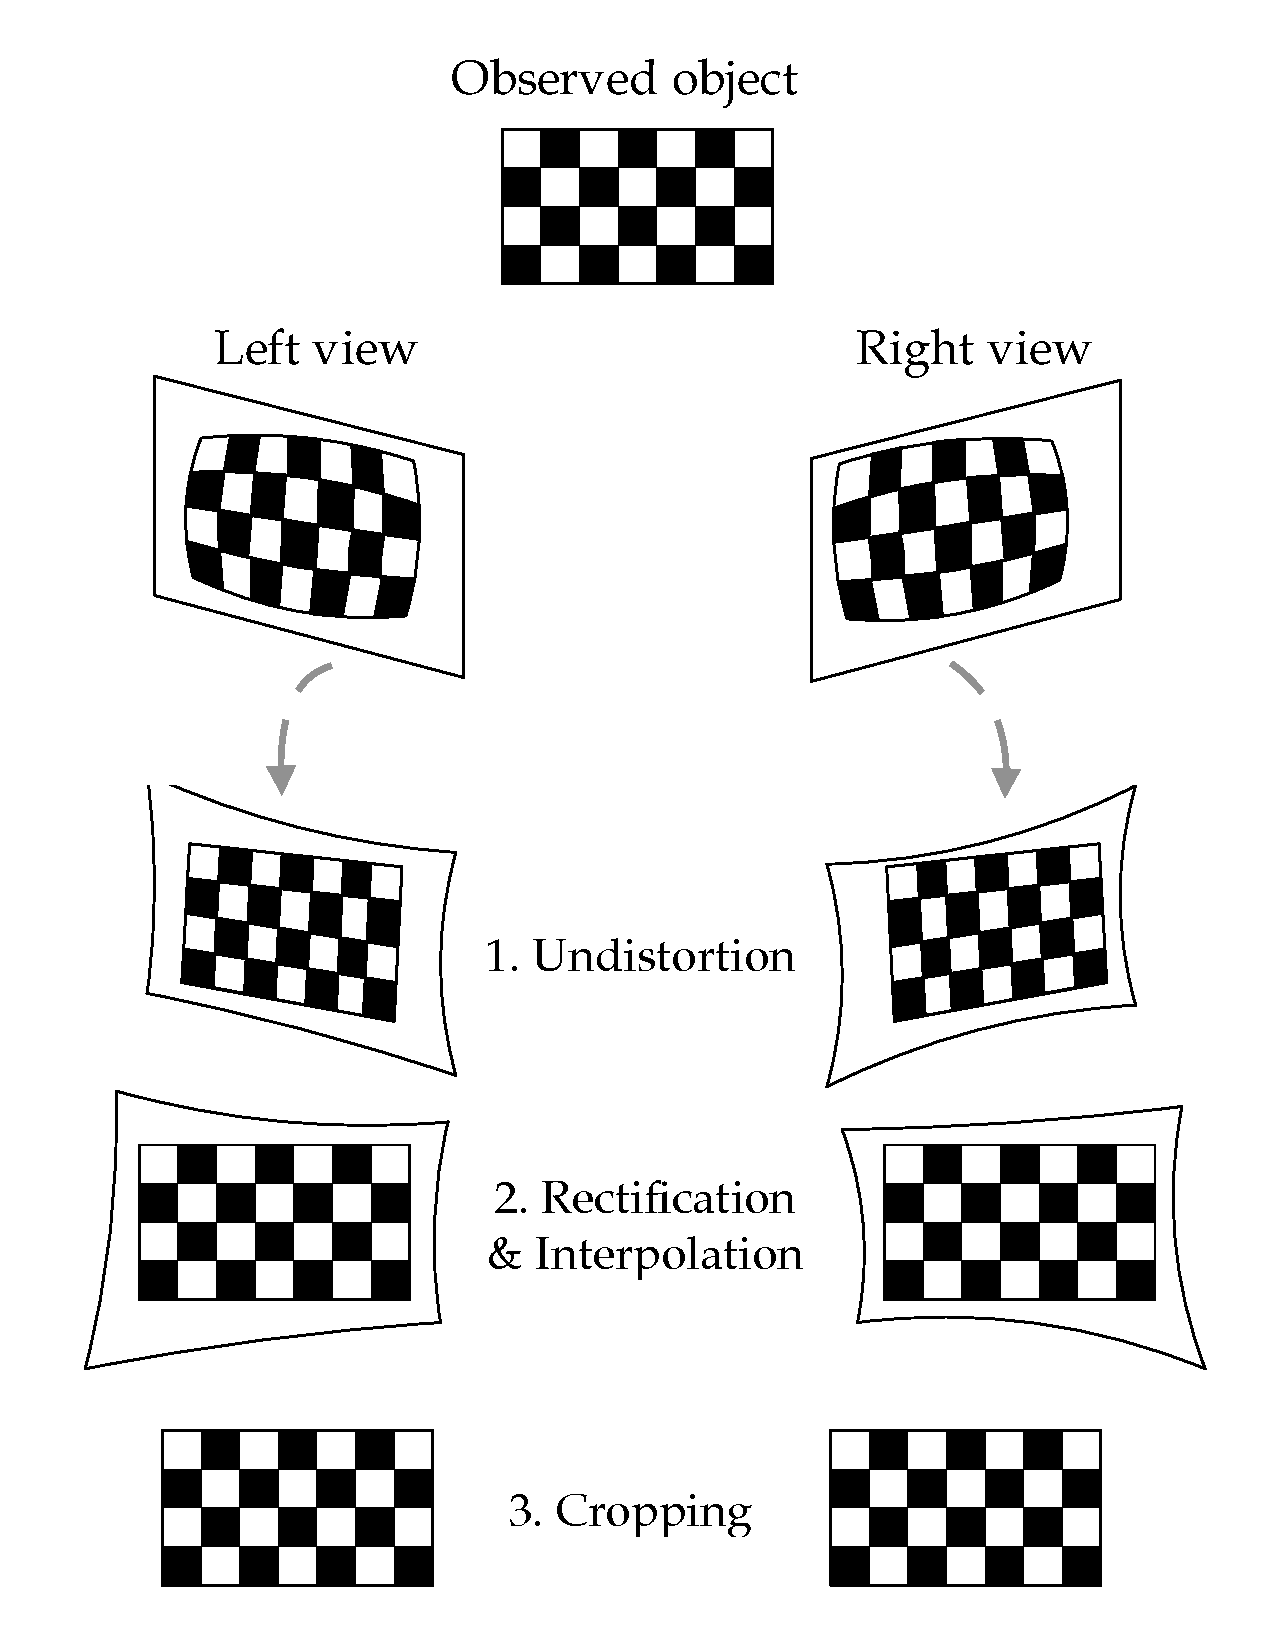
\includegraphics[width=0.75\textwidth]{classical-vo/stereo_rectification}
        \caption{Rectification and undistortion process. Figure adapted from \cite{florez2010}.}
         \label{fig:vo_undistort_recitfy}
	 \end{subfigure}
	 \begin{subfigure}[b]{0.48\textwidth}
         \centering
     		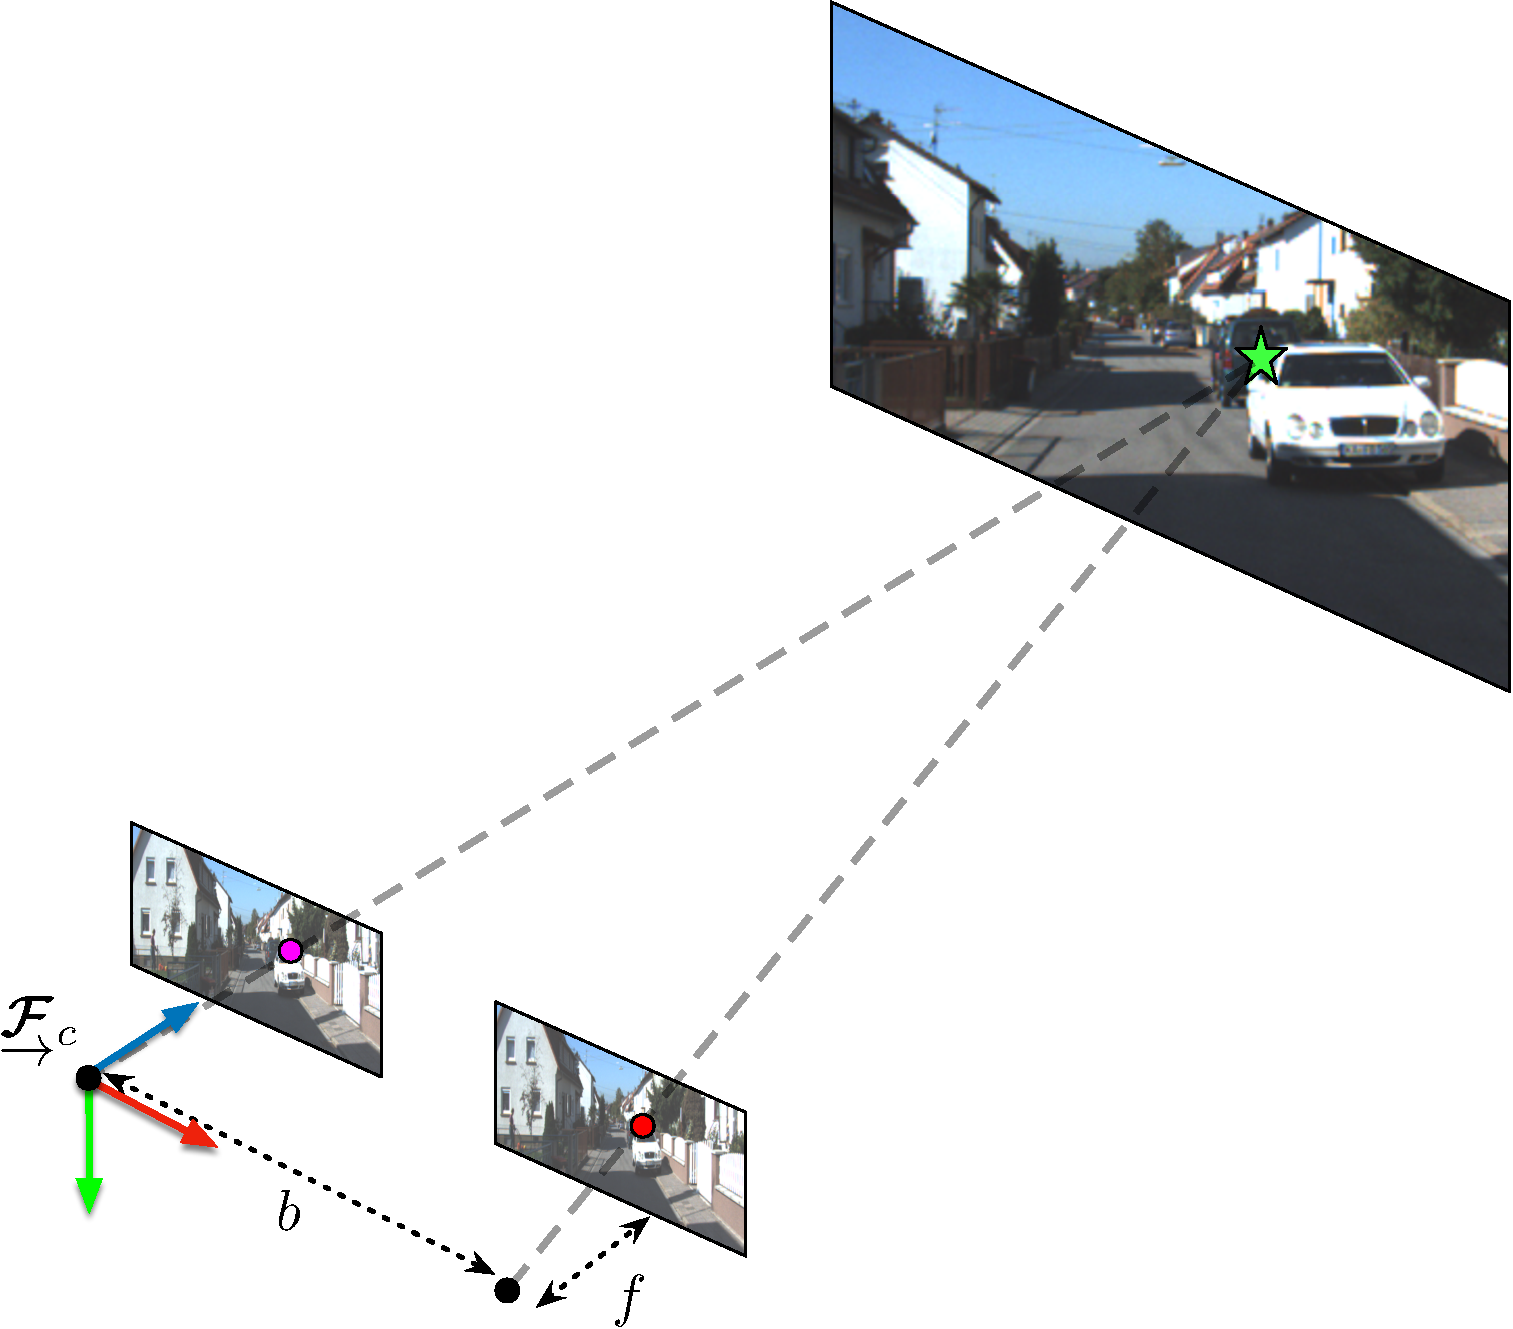
\includegraphics[width=0.98\textwidth]{classical-vo/stereo_camera}
			\caption{Ideal stereo camera.}
			 \label{fig:vo_stereo_camera}
     \end{subfigure}
    \caption{We pre-process stereo images (left) to simulate an ideal stereo camera (right).}
        \label{fig:vo_preprocessing}
\end{figure}
The preprocessing stage consists of two major steps. First, we use a lens model to undistort each stereo image. Second, we use the stereo camera calibration (i.e., the intrinsic parameters of each camera and the extrinsic parameters defining the transform $\Transform \in \LieGroupSE{3}$ between the two camera reference frames), to \textit{rectify, interpolate and crop} the pair of images such that we can assume a \textit{ideal frontoparallel stereo camera} model with a single focal length (\Cref{fig:vo_preprocessing}). That is, a stereo camera in which we can assume that any feature in one camera can be found in the same vertical location in the other (i.e., the epipolar line is horizontal). We assume the lens model, intrinsic and extrinsic parameters are constant and given by the dataset, or defined by a calibration process prior to data collection (e.g., given by the calibration tool detailed in \cite{Furgale2013-sl}).

\subsection{Data Association}
\label{sec:vo_data_extraction}
\subsubsection{Feature Extraction and Matching}
 
\begin{figure}[h!]
\begin{center}
		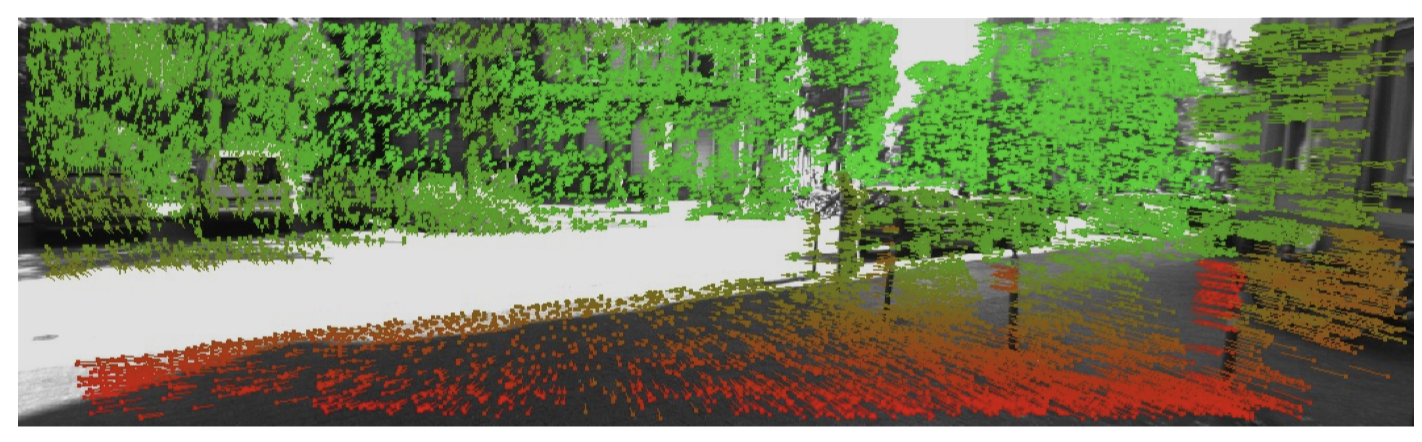
\includegraphics[width=0.99\textwidth]{classical-vo/libviso2_scan}
		\caption{Feature tracking using \textsc{viso2}, taken from \cite{Geiger2011-xe}. Colours correspond to depth.}
  	\label{fig:vo_feature_tracking}
\end{center}
\end{figure}
Although a number of different types of indirect feature extraction and matching methods have been presented in the literature (e.g., \textsf{SIFT}, \cite{lowe_object_1999} or \textsf{ORB}, \cite{rublee2011orb}), we choose to use the \textsf{viso2} \citep{Geiger2011-xe} algorithm due to its computationally efficiency (it can extract thousands of matches in milliseconds on modern hardware) and its use of a motion model that facilitates matching with sequential images. Briefly, \textsf{viso2} features are extracted using blob and corner masks with non-minimum and non-maximum suppression. Unlike other features detectors that do not assume a particular camera motion, \textsf{viso2} assumes a smooth camera trajectory that permits fast matching through a simple sum-of-absolute-difference error metric based on Sobel filter responses. Features are matched across a stereo-pair and forward in time with a consistency check to ensure that a single feature exists all four images in two stereo camera poses. 
\subsubsection{Ideal Stereo Camera Model}
We model each feature extracted by \textsf{viso2} as a three-dimensional point landmark that can be expressed (in homogeneous coordinates) in the camera frame, $\CoordinateFrame{c}$, as
$\HomogeneousPoint{i}{c} \in
\HomogeneousNumbers[3]$.  Our ideal stereo camera model, $\ProjectionFunction(\cdot)$,
projects $\HomogeneousPoint{i}{c}$ into image space coordinates as
 \begin{equation}
	\ImageLandmark{i}{c} = \bbm u_l \\ v_l \\ d  \ebm  
  =\ProjectionFunction(\HomogeneousPoint{i}{c}) =  \ProjectionFunction(\bbm x \\ y \\ z \\ 1 \ebm) = 
   \Matrix{M} \frac{1}{z} \HomogeneousPoint{i}{c},
\end{equation}
where
\begin{equation}
\Matrix{M} = \bbm f & 0 & c_u & 0 \\ 0 & f & c_v & 0 \\ 0 & 0 & 0 & fb \ebm.
\end{equation}
Here, $\{c_u, c_v\}$, $f$, and $b$ are the principal points, focal
length and baseline of the stereo camera respectively (computed through intrinsic and extrinsic calibration) and $d \definedtobe u_l - u_r$ is the \textit{disparity} of the feature. Note that in this
formulation, the stereo camera frame is in the left optical centre. Given $\ImageLandmark{i}{c}$, we also define the inverse operation, $\ProjectionFunction^{-1}(\cdot)$ (triangulation) as:
 \begin{equation}
	\HomogeneousPoint{i}{c} = \bbm x \\ y \\ z \\ 1 \ebm =  \ProjectionFunction^{-1}\left( \bbm u_l \\ v_l \\ d \ebm \right) =  \bbm  \frac{b}{d}(u_l - c_u) \\ \frac{b}{d}(v_l - c_v) \\ \frac{b}{d} f \\ 1 \ebm.
\end{equation}



\subsubsection{Outlier Rejection}
Given $N_t$ feature \textit{tracks} (i.e., the image locations of matching features across time), $\{\ImageLandmark{i}{c_0}, \ImageLandmark{i}{c_1}\}_{i=1}^{N_t}$, we filter out any \textit{outliers} by applying three-point random sample consensus algorithm (RANSAC, \cite{fischler1981random}) based on an analytic solution to the six degree-of-freedom motion \citep{Umeyama1991-ws} (refer to Appendix \ref{app:appendix_vo} for more details).
  
\subsection{Maximum Likelihood Motion Solution}
Finally, we compute the rigid-body transform between to stereo camera frames using maximum likelihood estimation. We define the rigid-body transform, $\Transform_t \in\text{SE}(3)$, to be the rigid-body transform between two subsequent stereo camera poses, 
$\CoordinateFrame{c_0}$ and  $\CoordinateFrame{c_1}$, 
\begin{equation}
	\Transform_t = \Transform_{c_1w} \Transform^{-1}_{c_0w},
\end{equation}
where $\CoordinateFrame{w}$ is a predefined world frame. For each track, $(\ImageLandmark{i}{c_0}, \ImageLandmark{i}{c_1})$, we define an error function, $\Vector{e}_{i,t}(\Transform_t, \ImageLandmark{i}{c_0}, \ImageLandmark{i}{c_1})$, that relates the rigid transform to these stereo feature matches. For notational clarity, we will refer to this term as simply $\Vector{e}_{i}(\Transform_t)$ with the dependence on the track implied. Next, we assume that these errors are corrupted by zero-mean independent Gaussian noise with the covariance, $\Matrix{\Sigma}_{i,t}$;
 \begin{equation}
  \Vector{e}_{i}(\Transform_t) \sim
 \NormalDistribution\left(\Vector 0, \GeneralCovariance_{i,t}\right). 
\end{equation}
Under this noise model, the maximum likelihood transform, $\Transform^*_t$, is given by 
\begin{equation}
\label{eq:vo_objective}
  \Transform_t^* = \ArgMax{\Transform\in\text{SE}(3)}\prod_{i=1}^{N_t} p(\Vector{e}_{i}(\Transform_t)) = \ArgMin{\Transform\in\text{SE}(3)} \frac{1}{2} \sum_{i=1}^{N_t} 
  \Transpose{\Vector{e}_{i}(\Transform_t)} \GeneralCovariance_{i,t}^{-1} \Vector{e}_{i}(\Transform_t).
\end{equation}
We will define the error function in two different ways.

\subsubsection{Point Cloud Error}
\label{sec:vo_point_cloud}
First, we can follow classical approach \citep{Maimone2007-tc} and define $ \Vector{e}_{i}(\Transform_t) $ based on a three-dimensional point cloud error. To do this, we invert our stereo camera model to triangulate pairs of points in each frame, $\HomogeneousPoint{i}{c_0} = \ProjectionFunction^{-1}(\ImageLandmark{i}{c_0})$ and $\HomogeneousPoint{i}{c_1} = \ProjectionFunction^{-1}(\ImageLandmark{i}{c_1})$, and then define a three-dimensional error,
\begin{align}
	 \Vector{e}_{i}(\Transform_t) = \Matrix{D}(\HomogeneousPoint{i}{c_1} - \Transform_t \HomogeneousPoint{i}{c_0}) \in \Real{}^3,
\end{align}
where $\Matrix{D} = \bbm \IdentityMatrix_{3\times3} & \Vector{0} \ebm \in \Real{}^{3\times4}$ converts homogenous coordinates into Euclidian coordinates.

\noindent We can then follow \cite{Maimone2007-tc} and assume each stereo projection is corrupted by additive Gaussian noise,
\begin{equation}
\ImageLandmark{i}{c} \sim \NormalDistribution\left(\bar{\Vector{y}}_{i,c}, \ImageLandmarkCovariance{i}{c} \right), 
\end{equation}  
and compute a density on the error function itself through first order noise propagation. This gives the density
 \begin{equation}
  \Vector{e}_{i}(\Transform_t) \sim
 \NormalDistribution\left(\Vector 0, \GeneralCovariance_{i,t} \right), 
\end{equation}
where
\begin{equation}
	\GeneralCovariance_{i,t} = \Matrix{D}\Matrix{G}_{i,c_1} \ImageLandmarkCovariance{i}{c_1}  \Matrix{G}_{i,c_1}^\Tr \Matrix{D}^\Tr + 
 \Matrix{D}\Transform_t \Matrix{G}_{i,c_0}  \ImageLandmarkCovariance{i}{c_0} \Matrix{G}_{i,c_0}^\Tr  \Transform_t^\Tr \Matrix{D}^\Tr,
\end{equation}
with
$\Matrix{G}_{i,c} = \at{\PartialDerivative{\ProjectionFunction^{-1}}{\Vector{y}}}{\ImageLandmark{i}{c}}$.

\subsubsection{Reprojection Error}
\label{sec:vo_reprojection}
Alternatively, we can represent reprojection errors in the second frame directly as
\begin{equation}
  \Vector{e}_{i}(\Transform_t)  = \ImageLandmark{i}{c_1} - \ProjectionFunction( \Transform_t 
    \ProjectionFunction^{-1}( \ImageLandmark{i}{c_0} ) ),
   \label{eq:image_error}
\end{equation}
\noindent and assume the following simple noise model
 \begin{equation}
  \Vector{e}_{i}(\Transform_t) \sim \NormalDistribution\left(\Vector 0, \GeneralCovariance_{i,t} \right) = 
 \NormalDistribution\left(\Vector 0,  \ImageLandmarkCovariance{i}{t}\right), 
\end{equation}
where the subscript $t$ in $\ImageLandmarkCovariance{i}{t}$ indicates that this measurement covariance refers to the reprojection error that involves a temporal track.

Importantly, \cite{Sibley2007} show that using reprojection error results in less biased estimates for long-range stereo triangulation (when compared to point cloud error). Consequently, we favour this latter formulation in the large majority of our work (the one exception being the initial work on isotropic PROBE described in Appendix \ref{app:appendix_probe_knn}).

\subsubsection{Solution via Gauss-Newton Optimization}
\label{sec:vo_gauss_newton}
 In either case, we have now defined a weighted nonlinear least squares problem which can be solved iteratively using
standard techniques. For our purposes, we opt to use Gauss-Newton optimization and follow \cite{Barfoot2017-ri} to optimize constrained poses.

Namely, at a given iteration $n$, we linearize the error function $\Vector{e}_{i}(\Transform_t)$, about an operating point $\Transform_t^{(n)} \in \LieGroupSE{3}$, which results in a quadratic approximation to \Cref{eq:vo_objective}. We follow \Cref{sec:math_perturbations} and use the left perturbations $\delta\Vector{\xi}^\ell \in\RealNumbers[6]$:
\begin{equation}
  \Transform_t = \MatExp{\delta\Vector{\xi}^\ell} \Transform_t^{(n)} \approx (\IdentityMatrix + \delta\Vector{\xi}^{\wedge}) \Transform_t^{(n)}.
\end{equation}
where we have dropped the perturbation superscript for brevity. This allows us to transform \Cref{eq:vo_objective} into a linear least squares objective in $\delta\Vector{\xi}$:
\begin{equation}
\label{eq:vo_linleastsquares}
  \mathcal{L}(\delta \Vector{\xi}) = \frac{1}{2}\sum_{i=1}^{N_t} 
  \Transpose{\left(\Vector{e}_{i}
  - \Matrix J_{i} \delta\Vector{\xi}\right)}
\GeneralCovariance_{i}^{-1}
 \left(\Vector{e}_{i}
 - \Matrix J_{i} \delta\Vector{\xi}\right)
  \end{equation}
where $\Matrix J_{i} = \at{\PartialDerivative{\Vector{e}_i}{\delta \Vector{\xi}}}{\Transform_t^{(n)}}$, $\Vector{e}_{i} = \Vector{e}_{i}(\Transform_t^{(n)})$, and $\GeneralCovariance_{i} =  \GeneralCovariance_{i,t}(\Transform_t^{(n)})$. 
The minimum to this objective can be solved for analytically by solving the normal equations. This results in the optimal parameters,  
\begin{equation}
  \delta\Vector{\xi}^{\star} = 
  \left( \sum_{i=1}^{N_t} \Transpose{\Matrix J}_{i}
  \GeneralCovariance_{i}^{-1} \Matrix J_{i} \right)^{-1}
  \sum_{i=1}^{N_t} \Transpose{\Matrix J}_{i}
  \GeneralCovariance_{i}^{-1} \Vector{e}_{i}. 
\label{eq:least-squares-iteration}
\end{equation}
Given $\delta\Vector{\xi}^{\star}$, we can update the operating point using the constraint-sensitive update
\begin{equation}
  \Transform_t^{(n+1)} = \MatExp{\delta\Vector{\xi}^{\star}} \Transform_t^{(n)}, \label{eq:vo_se3_update}
\end{equation}
and iterate until convergence. See Appendix \ref{app:appendix_vo}
for more details and an analytic expression for $\Matrix J_{i}$. 
There are many reasonable choices for both the initial transform
$\Transform_t^{(0)}$ and for the conditions under which we terminate
iteration. For most visual odometry applications, it suffices to initialize the estimated transform to identity, and iteratively
perform the update given by \Cref{eq:vo_se3_update} until we see a relative change in
the squared error of less than one percent after an update. 

%\newpage
%\section{Pose Graph Optimization}
%
%\begin{wrapfigure}{r}{0.4\textwidth}
%  \vspace{-20pt}
%  \begin{center}
%	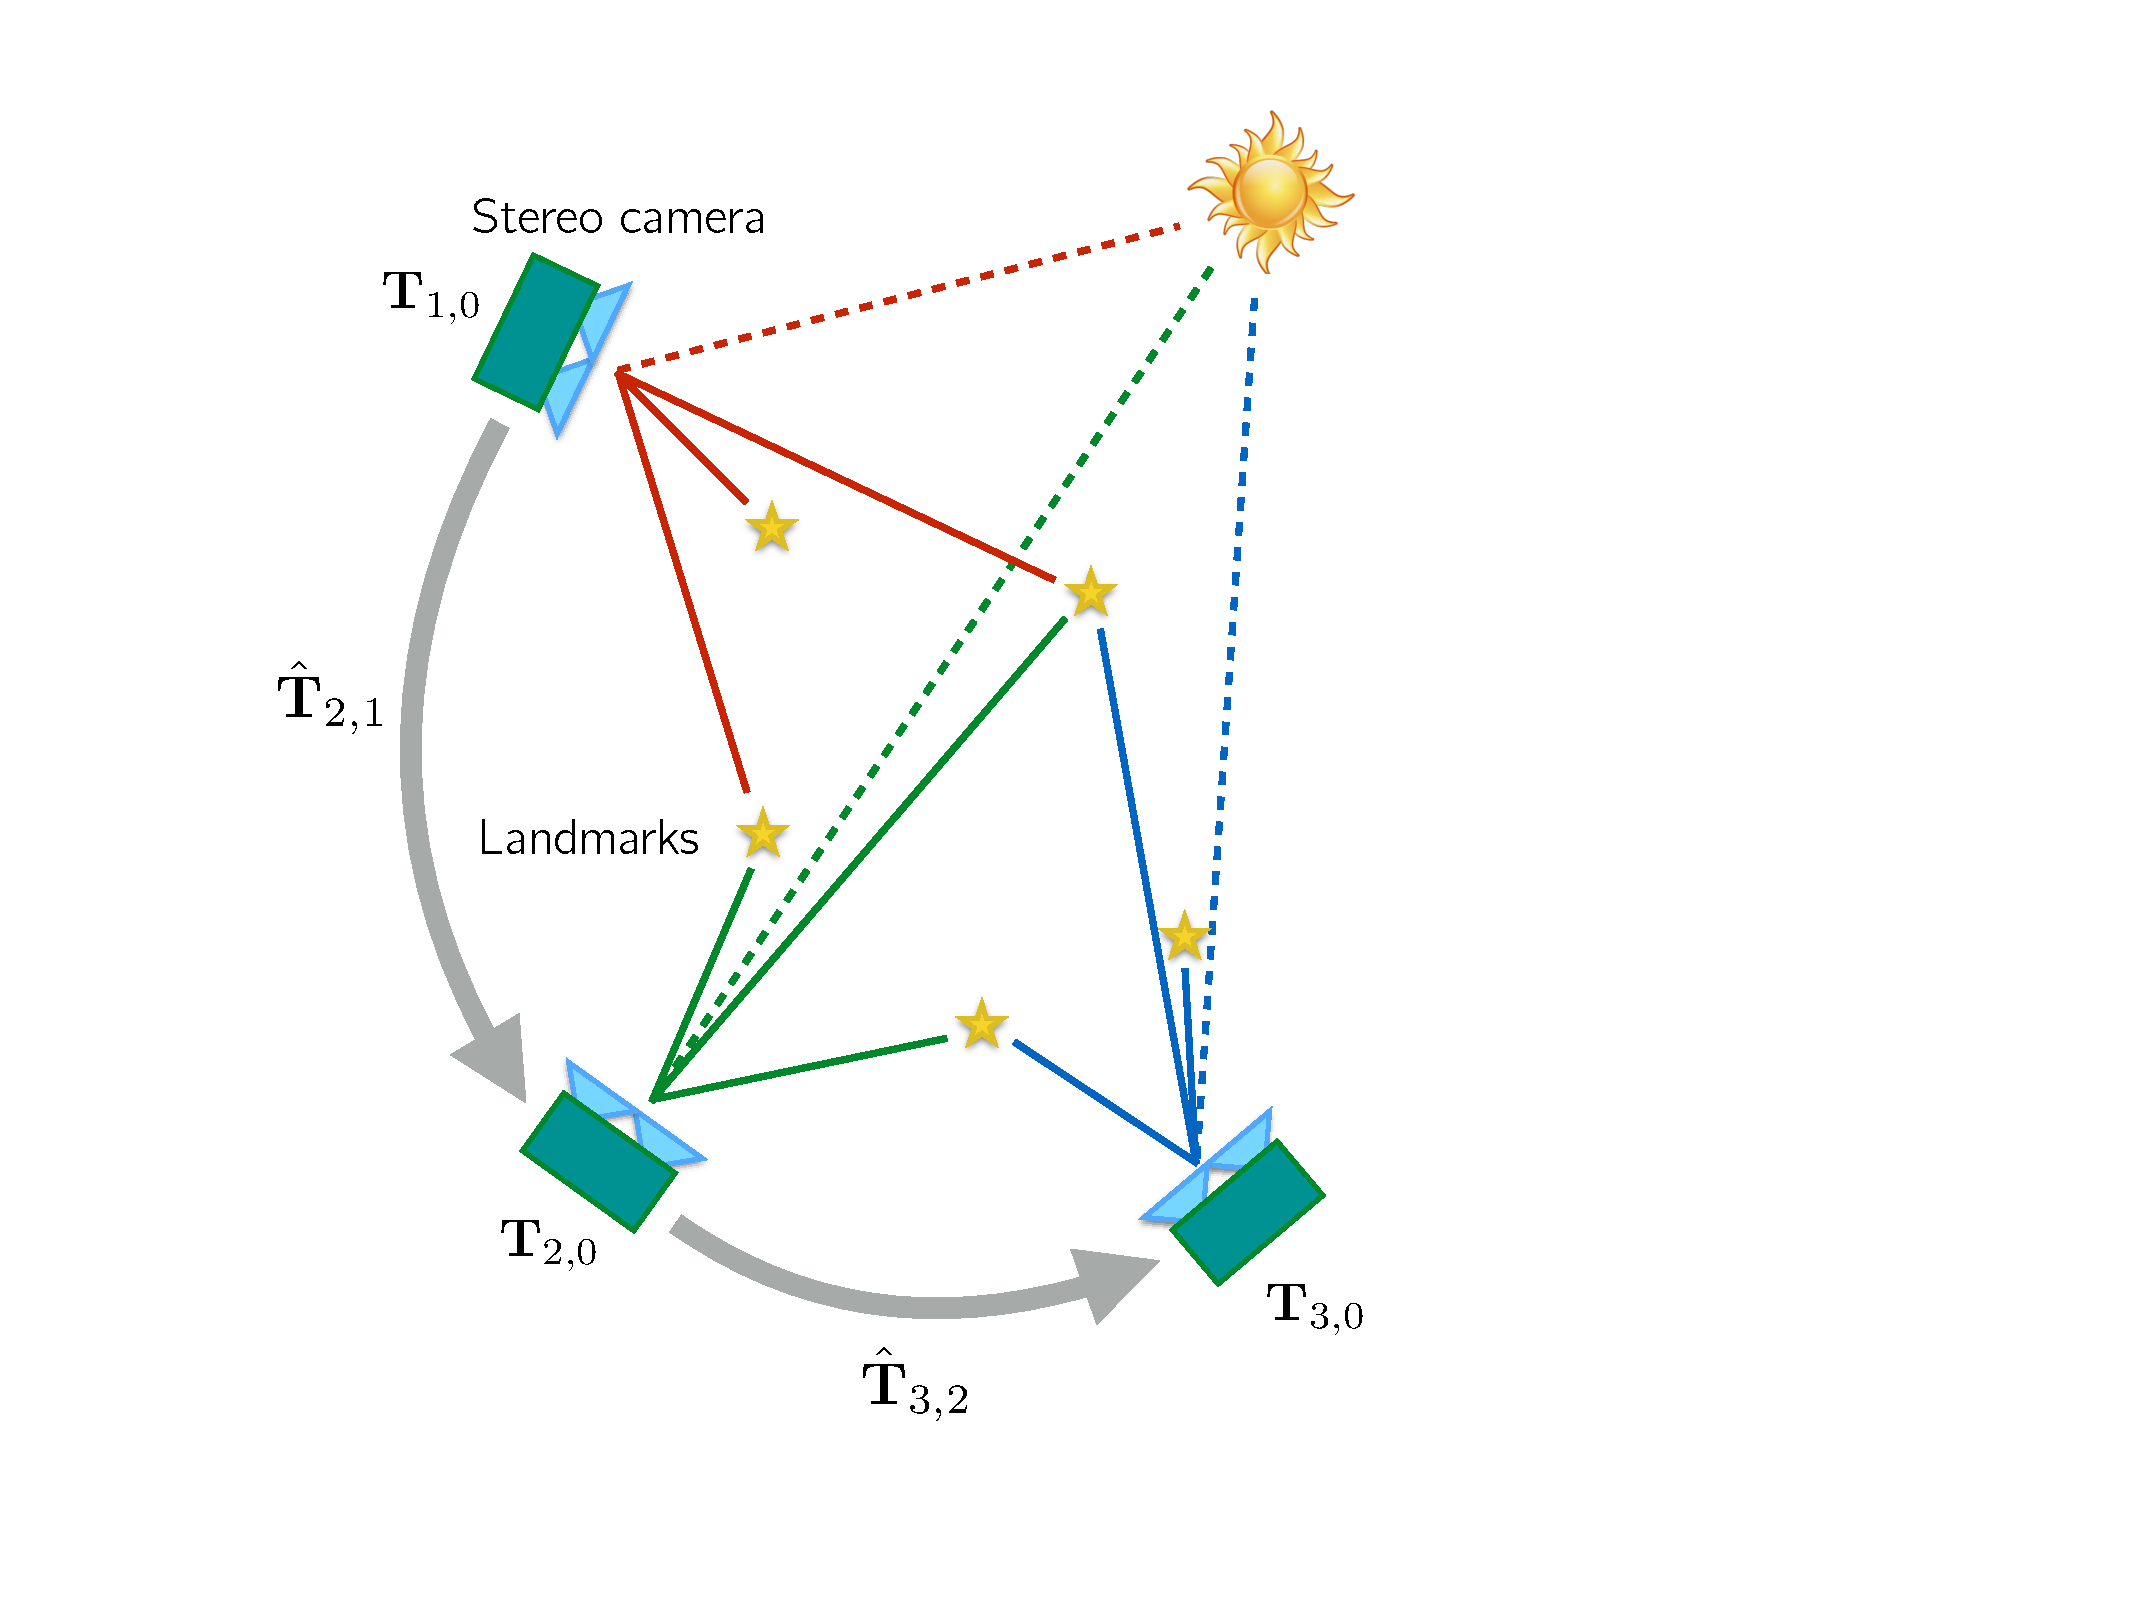
\includegraphics[width=0.38\textwidth]{classical-vo/pose_graph.pdf}
%  \end{center}
%    \vspace{-20pt}
%	\label{fig:math_pose_graph}
%	\caption{The formulation of pose graph relaxation can incorporate different probabilistic \textit{factors} that constrain each camera pose.}
%\end{wrapfigure} 
%
%
%we fused our probabilistic rotation regression with classical stereo visual odometry using pose graph relaxation implemented with the help of a Python-based factor graph library which we will publicize after the review process. Using that framework, we solved
%\begin{align}
%	\Transform_{1,w}^*, \Transform_{2,w}^* &= \ArgMin{\Transform_{1,w}, \Transform_{2,w}\in\text{SE}(3)}\mathcal{L}(\Estimate{\Transform}_{2,1}, \Estimate{\Rotation}_{2,1}) \\ & = \ArgMin{\Transform_{1,w}, \Transform_{2,w}\in\text{SE}(3)} \Vector{\xi}_\text{1,2}^\Tr \Matrix{\Sigma}^{-1}_\text{vo} \Vector{\xi}_\text{1,2} + \Vector{\phi}_\text{1,2}^\Tr \Matrix{\Sigma}^{-1}_{\text{hn}} \Vector{\phi}_\text{1,2} 
%\end{align}
%where
%\begin{equation}
%	\Vector{\xi}_\text{1,2} =  \MatLog{\left(\Transform_{2,w} \Transform_{1,w}^{-1} \right)\Estimate{\Transform}_{2,1}^{-1}},
%\end{equation}
%\begin{equation}
%	\Vector{\phi}_\text{1,2} =  \MatLog{\left(\Rotation_{2,w} \Rotation_{1,w}^{T} \right)\Estimate{\Rotation}_{2,1}^{T}},
%\end{equation}
%and $\Estimate{\Transform}_{2,1}$, $\Matrix{\Sigma}_\text{vo}$ and $\Estimate{\Rotation}_{2,1}$, $\Matrix{\Sigma}_{\text{hn}}$ were provided by our classical estimator and the HydraNet network respectively. Note that $\Matrix{\Sigma}_{\text{hn}} \in \Real^{3 \times 3} \geq 0$ while $\Matrix{\Sigma}_{\text{vo}} \in \Real^{6 \times 6} \geq 0 $. We also overload the logarithm function, $\MatLog{\cdot}$ to represent both $\LieGroupSE{3}$ and $\LieGroupSO{3}$ logarithmic maps as necessary. To account for gauge freedom, we fixed the first transformation to identity, $\Transform_{1,w} = \IdentityMatrix$, and initialized $\Transform_{2,w}$ to  $\Estimate{\Transform}_{2,1}$.  After convergence, we composed the final frame-to-frame estimate as $ \Transform_{2,1}^* =  \Transform_{2,w}^*  \left(\Transform_{1,w}^*\right)^{-1} = \Transform_{2,w}^*$.
%



\section{Robust Estimation}
Since \Cref{eq:vo_linleastsquares} assigns cost values that grow quadratically with measurement error, it is very sensitive to outlier measurements that may persist through RANSAC.
A common solution to this problem is to replace the quadratic loss function with one that is less sensitive to large measurement errors \citep{MacTavish2015-wt}.
These robust cost functions are collectively known as M-estimators\footnote{M, for \textit{maximum-likelihood-type} since they generalize the basic maximum likelihood solution \citep{Barfoot2017-ri}.}, and many variants exist. Each uses a re-weighting function, $\rho(\cdot)$, to define robust least squares (RLS) objective,
\begin{equation}
	\label{eq:vo_robust_loss_problem}
  \Transform^*_{\text{RLS}} = \ArgMin{\Transform\in\text{SE}(3)}\sum_{i=1}^{N} 
  \rho\left(\sqrt{\Transpose{\Vector{e}_{i}} \GeneralCovariance_{i}^{-1} \Vector{e}_{i}}\right) = \ArgMin{\Transform\in\text{SE}(3)}\sum_{i=1}^{N} 
  \rho(\epsilon_i) = \ArgMin{\Transform\in\text{SE}(3)} \mathcal{L}_{\text{RLS}}(\Transform),
\end{equation}
where we have defined $\epsilon_i \definedtobe \sqrt{\Transpose{\Vector{e}_{i}} \GeneralCovariance_{i}^{-1} \Vector{e}_{i}}$ (and dropped the $t$ subscript for clarity). The basic idea with M-estimation is to use a $\rho(\cdot)$ that reduces the influence of large $\epsilon$ below that of the quadratic $\rho(\epsilon) = \frac{1}{2} \epsilon^2$. There are several examples of such functions, including,
\begin{align}
\rho(\epsilon) &= \left\{  	\begin{array}{ll}
		 \frac{c^2}{2} \log{\left(1 + \frac{\epsilon^2}{c^2}\right)}   & \mbox{Cauchy,} \\
		 \frac{1}{2} \frac{\epsilon^2}{c^2 + \epsilon^2}  & \mbox{Geman-McClure \citep{geman1992nonlinear},} \\
		 \\
		\left\{  	\begin{array}{ll}  \frac{\epsilon^2}{2} & \mbox{if} ~\epsilon < c \\
										c\epsilon - \frac{c^2}{2} & \mbox{if} ~ \epsilon \geq c \end{array}
																						 \right.   & \mbox{Huber \citep{huber1964robust}.} \\
	\end{array}
	\right.
\end{align}
where the constant $c$ can be set with reference to asymptotic efficiency relative to a unit Gaussian \citep{Holland1977}. To solve \Cref{eq:vo_robust_loss_problem}, it is common in the literature to apply the technique of \textit{iteratively reweighted least squares} (IRLS) \citep{Holland1977}. To do this, we define a new non-linear least squares minimization problem,
\begin{equation}
\Transform^*_{\text{IRLS}} = \ArgMin{\Transform\in\text{SE}(3)}\frac{1}{2} \sum_{i=1}^{N} 
\Transpose{\Vector{e}_{i}} \Matrix{M}_{i} \Vector{e}_{i} = \ArgMin{\Transform\in\text{SE}(3)} \mathcal{L}_{\text{IRLS}}(\Transform)
\end{equation}
where we define these new weights, $\Matrix{M}_{i}$, based on an \textit{influence function}, $\psi(\cdot)$ as
\begin{equation}
	\Matrix{M}_i = \frac{1}{\epsilon_i} \underbrace{\at{\PartialDerivative{\rho}{\epsilon}}{\epsilon_i}}_{\psi(\epsilon_i)} \GeneralCovariance_{i}^{-1},
\end{equation}
and solve it using the Gauss-Newton approach presented in \Cref{sec:vo_gauss_newton}. We claim that upon convergence, $\Transform^*_{\text{IRLS}}$ will also minimize \Cref{eq:vo_robust_loss_problem}. To see why, consider that
\begin{equation}
\PartialDerivative{\mathcal{L}_{\text{RLS}}}{\delta \Vector{\xi}} = 	\sum_i^N \PartialDerivative{\rho}{\epsilon_i} \PartialDerivative{\epsilon_i}{\Vector{e}_i} \PartialDerivative{\Vector{e}_i}{\delta \Vector{\xi}} = 	\sum_i^N \frac{1}{\epsilon_i} \PartialDerivative{\rho}{\epsilon_i} \Transpose{\Vector{e}_{i}} \GeneralCovariance_{i}^{-1} \PartialDerivative{\Vector{e}_i}{\delta \Vector{\xi}}, 
\end{equation} where he have used the fact that $\PartialDerivative{\epsilon_i}{\Vector{e}_i} = \frac{1}{\epsilon_i} 	\Transpose{\Vector{e}_{i}} \GeneralCovariance_{i}^{-1}$. Now using our definition of $\Matrix{M}_i$, we can write,
\begin{equation}
\PartialDerivative{\mathcal{L}_{\text{RLS}}}{\delta \Vector{\xi}}  = 	\sum_i^N \Transpose{\Vector{e}_{i}} \underbrace{\frac{1}{\epsilon_i} \PartialDerivative{\rho}{\epsilon_i}  \GeneralCovariance_{i}^{-1}}_{\Matrix{M}_i(\Transform)} \PartialDerivative{\Vector{e}_i}{\delta \Vector{\xi}} = \sum_i^N \Transpose{\Vector{e}_{i}} \Matrix{M}_i(\Transform) \PartialDerivative{\Vector{e}_i}{\delta \Vector{\xi}}, 
\end{equation} where we have made the dependence on $\Transform$ explicit. We could potentially proceed to set this gradient to $\Vector{0}$ and attempt to solve for an optimal update $\delta \Vector{\xi}$. However, due to $\Matrix{M}_i(\Transform)$, this may be difficult in general.  Instead, we note that if we evaluate $\Matrix{M}_i{(\Transform})$ at the current operating point, $\Transform^{(n)}$, (i.e., we \textit{re-weight} the loss) we are then left with the equivalent normal equations that solve $\PartialDerivative{\mathcal{L}_{\text{IRLS}}}{\delta \Vector{\xi}} = \Vector{0}$.

Furthermore, upon convergence, our solution to the iteratively re-weighted problem $\Transform^{(n)} = \Transform_\text{IRLS}^*$ will also minimize the robust objective \Cref{eq:vo_robust_loss_problem}, since we must have that,
\begin{equation}
	\at{\PartialDerivative{\mathcal{L}_{\text{IRLS}}}{\delta \Vector{\xi}}}{\Transform_\text{IRLS}^*} = \at{\PartialDerivative{\mathcal{L}_{\text{RLS}}}{\delta \Vector{\xi}}}{\Transform_\text{IRLS}^*} = \Vector{0}.
\end{equation}
 



\newpage
\section{Outstanding Issues}
Finally, we summarize (\Cref{tab:vo_outstanding_issues}) several limitations of the canonical visual odometry pipeline we have presented in this chapter. Namely, the issues of efficiency, systematic bias and homoscedastic uncertainty. For each limitation, we will show in this dissertation that we can build a pseudo-sensor that addresses it for a particular environment (defined by the training data).

\begin{table}[h!]
	\caption{Issues that can be addressed by pseudo-sensors.}	\begin{threeparttable}
	\begin{tabular}{m{0.68\textwidth}m{0.28\textwidth}}
		\toprule
		\textsc{Synopsis} & \textsc{Addressed by} \\ \midrule  
		\textbf{Computational efficiency}: classical VO pipelines face a difficult-to-optimize trade-off between using all of the information contained within image while still remaining computationally tractable.  & PROBE (\Cref{ch:probe}) , DPC (\Cref{ch:dpc}) , Sun-BCNN (\Cref{ch:sun-bcnn}), HydraNet (\Cref{ch:hydranet}) \\
		& \\
		\textbf{Systematic bias}: Stereo visual odometry can incur systematic bias through poor extrinsic or intrinsic calibration, stereo triangulation errors, poor feature \textit{spread} (i.e., concentration of features on one side of an image), and poor data association due self-similar textures. &  DPC (\Cref{ch:dpc}), HydraNet (\Cref{ch:hydranet}) \\
		& \\
		\textbf{Homoscedastic uncertainty}: Stationary, homoscedastic noise in observation models can often reduce the consistency and accuracy of state estimates. This is especially true for complex, inferred measurement models. &  DPC (\Cref{ch:dpc}) , Sun-BCNN (\Cref{ch:sun-bcnn}), HydraNet (\Cref{ch:hydranet})\\
		& \\
		\bottomrule
	\end{tabular}
	\label{tab:vo_outstanding_issues}
\end{threeparttable}
\end{table}


%
%
%\textbf{Adaptation to new environments}
%
%\begin{table}[h!]
%	\begin{threeparttable}
%	\begin{tabular}{m{0.68\textwidth}m{0.28\textwidth}}
%		\toprule
%		\textbf{Synopsis} & \textbf{Addressed by} \\ \midrule  
%		Traditional VO pipelines do little to adapt to new environments.
%. &  PROBE-GK, DPC-Net, HydraNet \\
%		& \\
%		\bottomrule
%	\end{tabular}
%\end{threeparttable}
%\end{table}

